\section{Realisierung}

\subsection{Programmierumgebung / Programmierrichtlinien}
Als Programmierumgebung wird Visual Studio 2022 verwendet. Die App basiert auf dem .net Framework 6.0. Die Programmierrichtlinien sind die Standard-C\#-Richtlinien.
\subsubsection{Verwendete NuGet-Pakete}
\begin{table}[H]
  \centering
  \setlength\extrarowheight{2pt}
    \begin{tabulary}{1.0\textwidth}{|L|m{10cm}|}
      \hline
      \rowcolor[HTML]{4473C5}\textbf{Paket}& \textbf{Beschreibung}\\
    \hline
    \textbf{FontAwesome6.Svg V1.1.0} & Wird für die Icons in der MenuBar verwendet.\\
    \hline
    \textbf{MaterialDesignMessageBox.SirTheta V1.1.3} & Eine Messagebox welche das Material Design Theme verwendet. Die Standard Messagebox passt nicht zu der sonst nach Material-Design aufgebauten Applikation. Dieses NuGet-Paket wurde von mir selber erstellt. Der Sourcecode dazu ist auf GitHub unter \href{https://github.com/sirtheta/MaterialDesignMessageBox}{https://github.com/sirtheta/MaterialDesignMessageBox} verfügbar und kann frei verwendet werden.\\
    \hline
    \textbf{MaterialDesignTheme V4.4.0} & Wird für die GUI-Darstellung verwendet. Enthält Material Design Templates und Styles für WPF Controls in .NET\\
    \hline
    \textbf{Microsoft.EntityFrameWorkCore V6.0.4} & Database-Mapper mit LINQ-Query Support. Wird für die Datenbankverwaltung verwendet\\
    \hline
    \textbf{Microsoft.EntityFrameWorkCore.SqlServer V6.0.4} & Microsoft SQL Server database provider für Entity Framework Core\\
    \hline
    \textbf{Notifications.Wpf.Core V1.4.0} & Toast notifications für WPF apps. Wird zum anzeigen von Toasts in der App verwendet \\
    \hline
\end{tabulary}
\caption{Verwendete NuGet-Pakete}
\end{table}

\subsection{Softwareaufbau}
Die Applikation wird komplett im MVVM-Pattern aufgebaut. MVVM steht für Model-View-ViewModel. Mit diesem Konzept wird das View über DataBinding an das ViewModel gekoppelt, welches dann wiederum mit dem Model kommuniziert. 

\begin{figure}[H]
  \begin{center}
    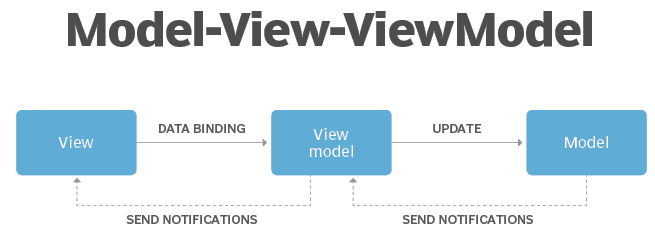
\includegraphics[width=0.6\linewidth]{content/images/mvvm.png}
    \caption{MVVM-Diagramm}
    \label{mvvm}
  \end{center}
\end{figure}

Somit besteht in der Applikation für jedes View ein ViewModel mit den entsprechenden Properties zum anbinden an das View.\\
Um die Applikation Mehrsprachig zu gestalten, wurden alle Texte in einer Ressourcen-Datei erfasst. Für jede Sprache die unterstützt werden soll, muss eine solche Datei angelegt werden. Beim Start der Applikation wird je nach Systemsprache die entsprechende Sprachdatei geladen. Hierzu wurde ein override der ''OnStartup'' Methode gemacht, welches die Sprachdatei lädt. (Siehe App.xaml.cs)



\subsection{GUI-Implementierung}
Das Main-GUI ist in drei Bereiche durch ein Grid aufgeteilt, wie in der Grafik \fref{guiGrid} zu sehen ist.

\begin{figure}[H]
  \begin{center}
    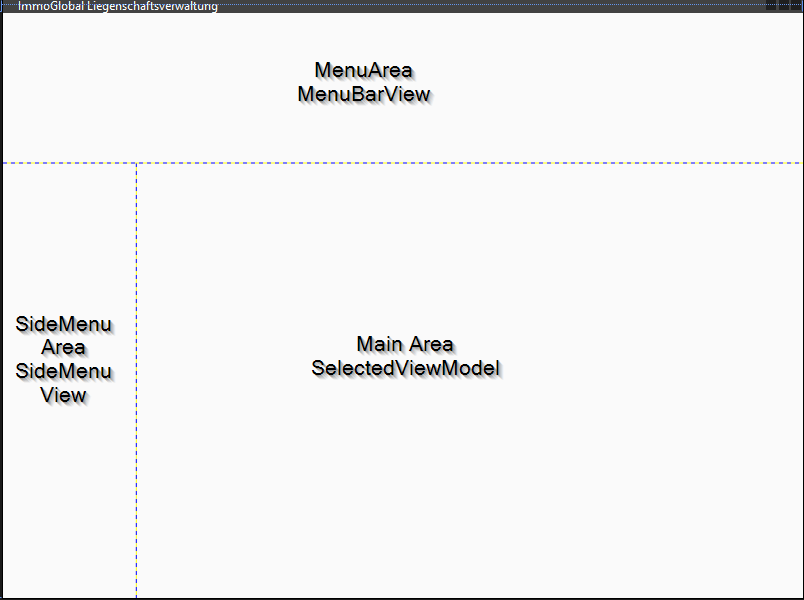
\includegraphics[width=0.6\linewidth]{content/images/MainGuiGrid.png}
    \caption{Main GUI Grid Aufbau}
    \label{guiGrid}
  \end{center}
\end{figure}
Die MenuArea und die SideMenuArea werden beim Start der Applikaton durch das entsprechende ViewModel abgefüllt und nicht mehr neu geladen. Im seitlichen Menü werden je nach dem welches ViewModel in der MainArea geladen ist, die Buttons entsprechend angepasst und in der Menu Bar wird das Icon rot eingefärbt wenn das entsprechende ViewModel in der MainArea geladen ist. So kann die Applikation sehr Dynamisch und übersichtlich gestaltet werden.
Alle Views bis auf das MainWindowView sind als UserControl definiert und können an beliebiger stelle in der Applikation eingebunden werden, was das wiederverwenden der Module deutlich vereinfacht.

\subsubsection{Namenskonzept für GUI-Komponenten}
Für das GUI werden verschieden Namen verwendet welche hier beschrieben werden.
\begin{itemize}
  \item \textbf{DetailsView:} Definiert kleinere Module für Detailanzeigen wie z.B. die Detailanzeige für den Mieter
  \item \textbf{Menu:} Definiert die Menus
  \item \textbf{Overview:} Definiert die Views für die Übersichten
  \item \textbf{Upsert:} Definiert die Views für Update und Insert, z.B wird ein View zum erstellen eines Mieters (Insert) und zum anpassen eines Mieters verwendet.
\end{itemize}


\subsection{Datenbankimplementierung und –anbindung}
\subsection{Testprotokoll}
